\chapter{ADCS}
\label{chapter:ADCS}

% small intro

% requirements + context -> what we have to do and for what

% DOT and pruning based on constraints + other subsystems

% \begin{itemize}
%     \item intro
%     \item requirements + constraints -> what we have to do -> scope
%     \item ADCS
%     \begin{itemize}
%         \item attitude determination
%         \begin{itemize}
%             \item DOT
%             \item pruning
%             \item one option left -> IMU
%         \end{itemize}

%         \item attitude control
%         \begin{itemize}
%             \item dot
%             \item model
%             \begin{itemize}
%                 \item reasoning to find out what we need and why
%             \end{itemize}
%             \item ref paper etc
%             \item method and assumptions
%             \item sensitivity analysis (inputs vs outputs)
%             \begin{itemize}
%                 \item constraints + dependencies from the other subsystems
%             \end{itemize}
%             \item conclusion -> final baseline
%             \begin{itemize}
%                 \item length
%                 \item n cables
%                 \item attachment radius
%                 \item damping
%                 \item DOT
%                 \item passive actuators
%                 \item final baseline -> what is preferred -> input for structural implementation
%                 \item dynamic insights
%                 \item MMOI
%                 \item symmetry
%                 \item aerodynamic configuration
%                 \item other preferences
%                 \item mass cables
%             \end{itemize}
%         \end{itemize}
%     \end{itemize}

%     \item conclusion
%     \begin{itemize}
%         \item final baseline
%         \item outputs
%         \item inputs for the other subsystems
%         \begin{itemize}
%             \item structures (all the above)
%             \item power (visibility, cable length)
%             \item communications -> processing both payload and imu onboard; also antenna?
%             \item GNC (IMU and absolute attitude)
%             \item ISRU (cable length?)
%             \item payload (radiometer) -> DH
%         \end{itemize}
%     \end{itemize}

% \end{itemize}

The VISTA aerobot is a suspended balloon–gondola system rather than a regular rigid spacecraft, hence its ADCS is not a standard three-axis pointing system. Instead, ADCS focuses on determining and tracking the local dynamic state of the gondola, including attitude, angular rates, oscillations, and post-deployment residual motion. Because no subsystem requires precise pointing, the main objective is to keep the motion bounded, observable, and compatible with the other subsystems. Furthermore, the dynamic behaviour of the gondola has to be assessed to correct the raw scientific measurements obtained by the payload, such as the variations in windspeed. Functions such as global navigation (GNC), altitude control (GNC), measurement numerical correction (C\&DH), deployment control (EDD), and structural verification (STR) remain outside the scope of ADCS. 

This chapter presents the process and rationale for selecting the ADCS configuration, which entails: attitude determination, attitude control/damping, and the dynamic configuration parameters (length of the suspension cables $L_{susp}$, the number of suspension cables $N_{susp}$, the attachment radius $r_{susp}$).

\section{ADCS Constraints, Interfaces and Design Drivers}
\label{sec: ADCS constraints, interfaces and design drivers}

The ADCS design is strongly driven by both the context of the mission and by the constraints imposed by the other subsystems. When it comes to the mission environment, classical attitude references become limited \cite{Cutts2022VenusAerobot}. Star trackers, sun, horizon and surfaces sensing become unreliable due tot the cloud scattering, while magnetic heading cannot be used due to the lack of Venusian magnetic field.

Regarding the subsystem interfaces, the Payload requires accurate attitude metadata for corrected scientific measurements (eg. wind sensor). However, no direct pointing is needed for the proper functioning of instruments. This also applies to the Communications subsystem by choosing omni-directional antennas. The GNC subsystem employs and IMU that can be shared with the ADCS if it is part of the chosen configuration. Furthermore, the Power subsystem requires a minimum cable length of $10$m to mitigate the obstruction of the solar panels, and longer is preferred. 

Moreover, the ADCS and Structures share significant parameters, as the structural configuration has a profound impact on the dynamic behaviour of the aerobot. The shared parameters include: gondola mass, CG position, inertia tensor, geometry, cable length, cable count etc. This complex relationship will be clarified throughout the next two chapters. Lastly, the design must also ensure it complies with the allocated technical budgets for mass, power, cost and data rate. Minimizing these resources is therefore desired. 

\section{Attitude Determination Configuration}
\label{sec: Attitude determination configuration}
\autoref{fig: DOT_ADCS_Attitude} present the design option tree for the Attitude Determination Configuration. Due to the unique mission constraints stated above (eg: cloud scattering, no magnetic field, distance to the Earth), significant pruning has been performed, highlighted in red. This resulted in 4 feasible options left: a 3-axis gyro (IS-1), a 3-axis accelerometer (IS-2), a 6-axis IMU (IS-3= IS-1 + IS-2) and attitude determination based on the Doppler navigation with the orbiter (RS-1). To maximize the attitude knowledge, a combination of the 4 options has been selected as the architecture, highlighted in green. 

The retained baseline is therefore a local inertial sensing approach based on a 6-axis IMU placed close to the gondola centre of gravity for accurate measurement of the intrinsic dynamic motion. Otherwise, additional terms ($\omega \cdot r_{CG-IMU}$) have to be accounted for. The gyroscopes provide angular-rate measurements for swing, yaw, spin, and torsional motion, while the accelerometers provide the 3-axis accelerations, aiding roll and pitch estimations relative to the local gravity and detecting the shocks experienced. As the gyroscope acquires only the relative attitude, which is subjected to IMU drift \cite{Frazier2022}, the orbiter is used to as an absolute reference during the contact times, by leveraging the Doppler technology selected in \autoref{chapter: guidance and navigation} by GNC. Furthermore, as the GNC subsystem also requires a 6-axis IMU architecture, it has been decided that ADCS and GNC will share the exact same low-drift configuration: 3 x Honeywell single axis QA-3000 \cite{HoneywellQA3000} for the accelerations and Safran STIM300 \cite{SafranSTIM300} for the 3-axis gyroscope, as recommended by \cite{Frazier2022}.

\begin{figure}
    \centering
    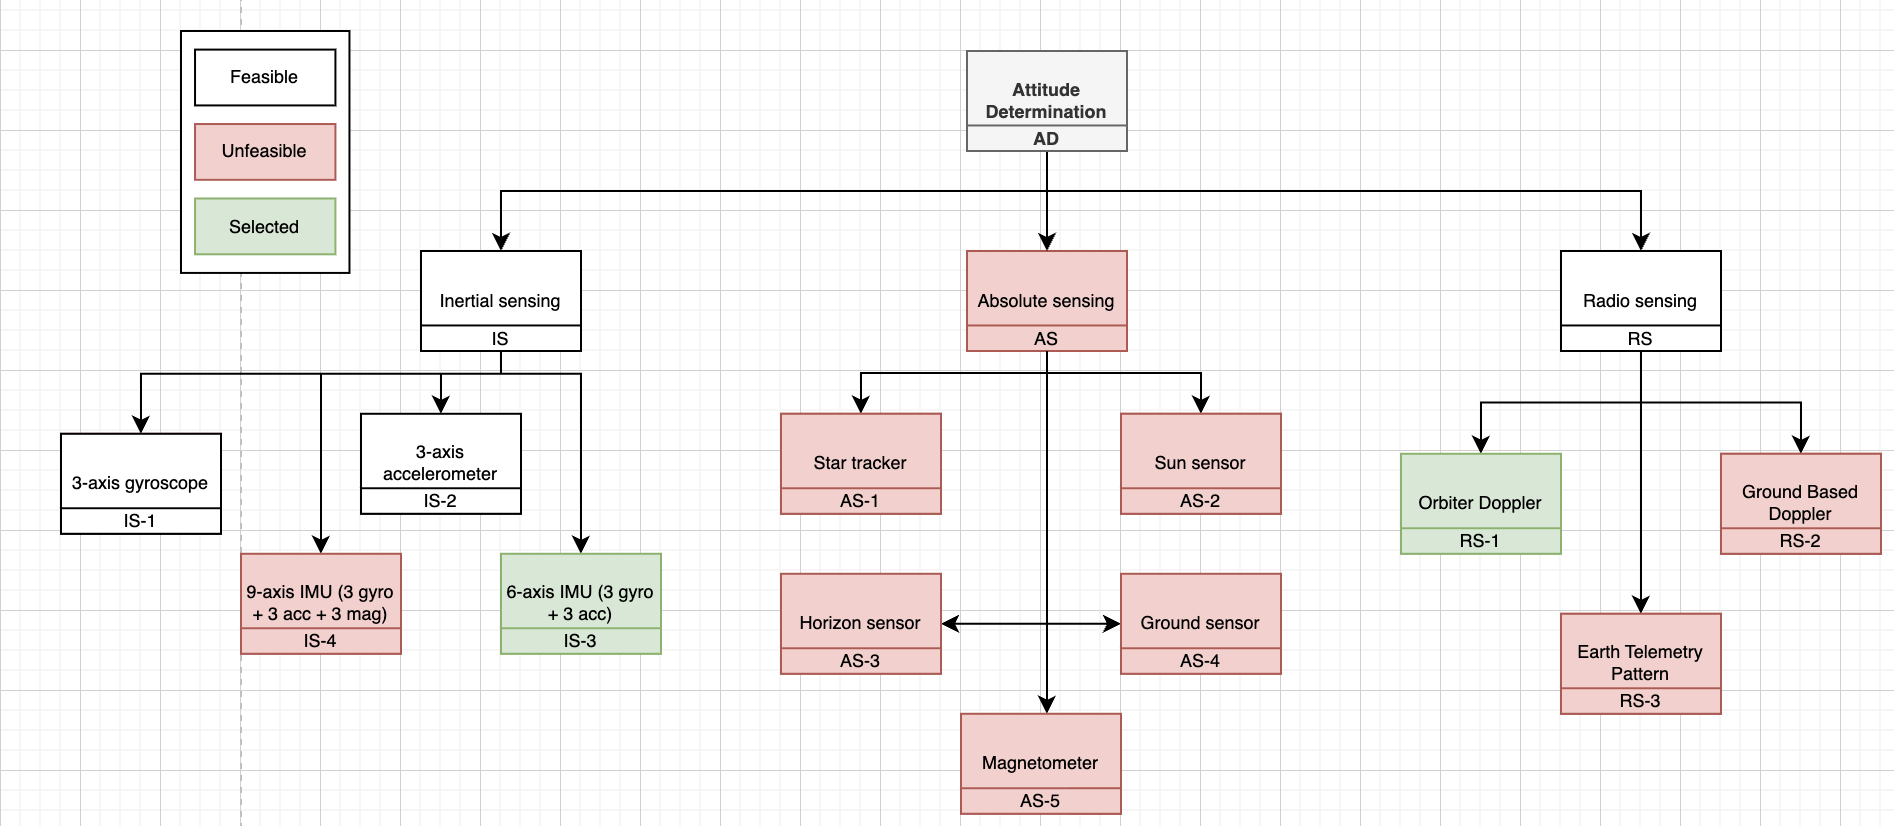
\includegraphics[width=0.9\linewidth]{fig/DOT_ADCS_ATTITUDE.png}
    \caption{Design Option Tree for the Attitude Determination Configuration}
    \label{fig: DOT_ADCS_Attitude}
\end{figure}
%
\section{Dynamic Modeling}
\label{sec: Dynamic Modeling}
The disturbances (aerodynamic gusts, wind shear, vertical winds, internal movements etc.) can excite two main dynamic behaviours throughout the mission: pendulum swing of the gondola beneath the balloon, and torsional oscillation of the gondola around the yaw axis. If the gondola mass distribution is not symmetric, pendulum and torsional motion may also become coupled \cite{Kassarian2021BalloonDynamics}. These behaviours matter because they affect payload measurement quality, structural load (cable tension), IMU range, sampling frequency and others.

\subsection{Methodology}
Informed preliminary design decisions can only be made by getting a better understanding of the complex dynamics of the system. For this, a simplified numerical model, presented in \cite{GithubVenusBalloonProject} has been created, aligned with the methods of Kassarian et al. \cite{Kassarian2021BalloonDynamics}. The suspended balloon-gondola system has been analyzed by dividing the suspension elements in multiple nodes, each with its own degrees of freedom: pendulum angle and torsional angle. Instantaneous snapshots for two different payload configurations are presented in \autoref{fig:gondola_sim}.

\begin{figure}[H]
    \centering

    \begin{subfigure}[b]{0.48\textwidth}
        \centering
        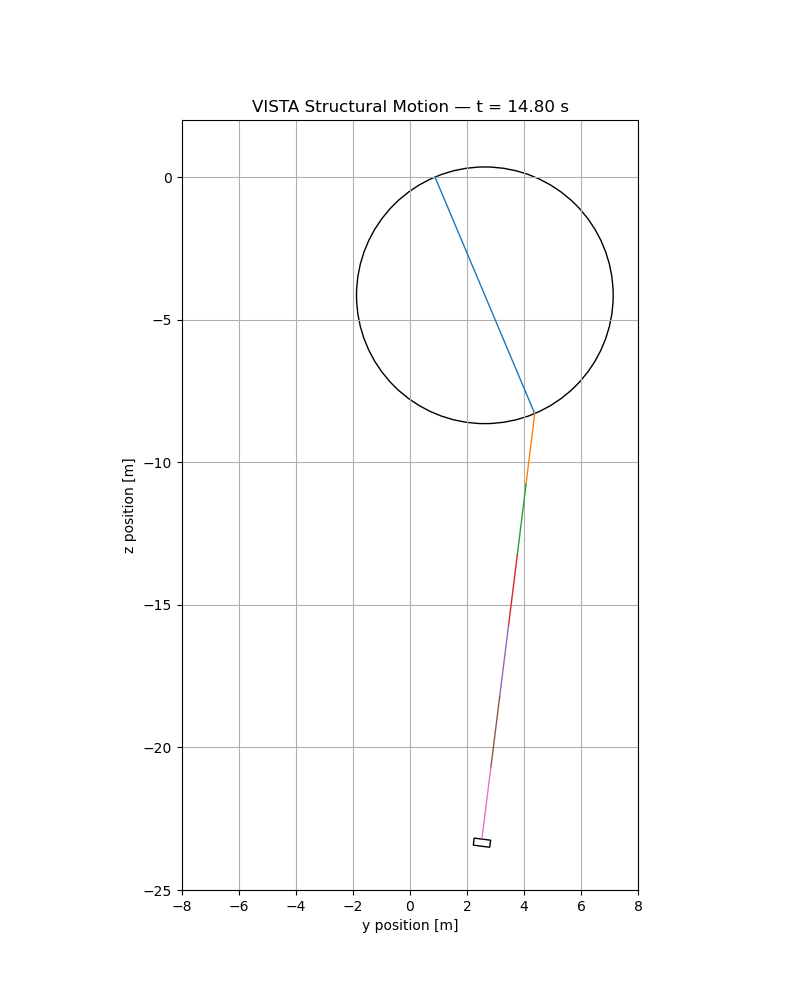
\includegraphics[width=\textwidth]{fig/Gondola_sim.png}
        \caption{Gondola structural simulation}
        \label{fig:gondola_sim}
    \end{subfigure}
    \hfill
    \begin{subfigure}[b]{0.48\textwidth}
        \centering
        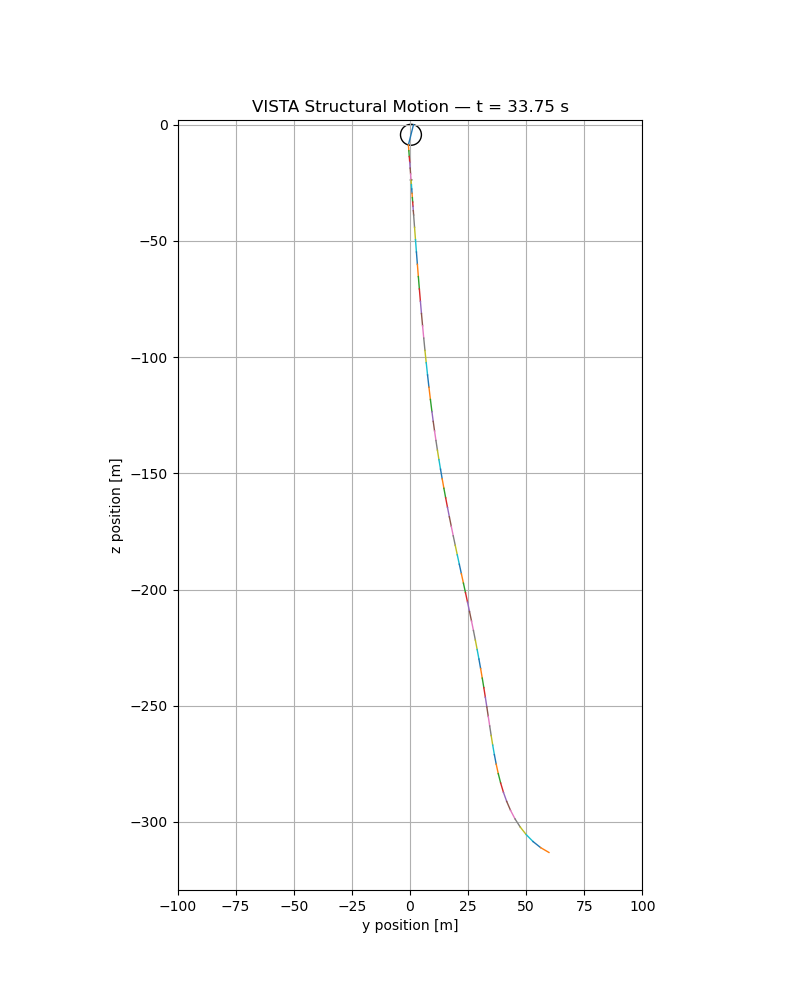
\includegraphics[width=\textwidth]{fig/tether_sim.png}
        \caption{Tether structural simulation}
        \label{fig:tether_sim}
    \end{subfigure}

    \caption{Dynamic simulation results for the gondola and tether configurations}
    \label{fig:struc_sims}
\end{figure}

The governing equations are 
\begin{equation}
    \mathbf{M}_x \ddot{\mathbf{x}} + \mathbf{C}_x \dot{\mathbf{x}} + \mathbf{K}_x \mathbf{x} = \mathbf{F}_x(t) \text{ and }
    \\
    \mathbf{M}_z \ddot{\mathbf{z}} + \mathbf{C}_z \dot{\mathbf{z}} + \mathbf{K}_z \mathbf{z} = \mathbf{T}_z(t)
\end{equation}
where $\mathbf{M}$, $\mathbf{C}$, and $\mathbf{K}$ are the mass, damping, and stiffness matrices for the pendulum/torsional oscillations, and $\mathbf{F}(t)$ represents the simplified disturbance inputs or initial conditions. For a detailed derivation of these equations, the reader is encouraged to delve into \cite{Kassarian2021BalloonDynamics}.

The model takes as inputs the disturbances and the architecture parameters and is used to compute the gondola maximum swing and yaw angles, angular rates, angular accelerations, natural frequencies, dominant periods, settling times, and a the maximum cable tension. It must be noted that the model relies on several assumptions, such small-angle approximations, gondola symmetry and damping modeled directly in the damping coefficients. These aspects will be refined in the further phases of the design.

\subsection{Sensitivity Analysis}
\label{subsec: Sensitivity Analysis}
A sensitivity analysis was performed to assess how the main suspension design parameters influence the dynamic response of the balloon–gondola system. The trends are compiled in \autoref{tab:adcs_sensitivity_trends}, providing valuable insights for the configuration selection from \autoref{sec: configuration selection}.


\begin{table}[htbp]
\centering
\caption{Sensitivity trends for increasing the main suspension design parameters.}
\label{tab:adcs_sensitivity_trends}

\renewcommand{\arraystretch}{1.35}

\begin{tabularx}{0.92\textwidth}{
>{\raggedright\arraybackslash}p{2.6cm}
>{\centering\arraybackslash}X
>{\centering\arraybackslash}X
>{\centering\arraybackslash}X
>{\centering\arraybackslash}X
>{\centering\arraybackslash}X
}
\toprule

\textbf{Input varied} &
\textbf{Period} &
\textbf{Amplitude} &
\textbf{Rate} &
\textbf{Settling time} &
\textbf{Tension} \\

\midrule

$L_{\mathrm{susp}}$
& \textit{I / I}
& \textit{E / I}
& \textit{NM / D}
& \textit{I / I}
& \textit{E / E} \\

$N_{\mathrm{cables}}$
& \textit{E}
& \textit{E}
& \textit{E}
& \textit{E}
& \textit{E} \\

$r_{\mathrm{susp}}$
& \textit{E / D}
& \textit{E / D}
& \textit{E / I}
& \textit{E / D}
& \textit{E} \\

\bottomrule
\end{tabularx}

\vspace{0.3cm}

\begin{minipage}{0.92\textwidth}
\footnotesize
\textit{For combined entries, the first trend refers to the pendulum response and the second to the torsional response.}
Legend: E = equal, I = increase, D = decrease, NM = non-monotonic.
\end{minipage}

\end{table}

The sensitivity results show that suspension length mainly controls the time scale of the suspended system. Increasing $L_{susp}$ increases the dominant pendulum and torsional periods and reduces the yaw-rate response, but it also increases settling time, angular amplitudes, and the physical balloon--gondola separation. The number of cables $N_{susp}$ has little effect on the global pendulum and torsional response, so its relevance is mainly structural: load sharing, redundancy, and deployment complexity. The attachment radius is the dominant torsional design variable. Increasing $r_{susp}$ stiffens the torsional mode and reduces twist amplitude, but it also increases yaw-rate response and torsional interface demand. Moreover, the layout of the gondola has also been analyzed. It was found that, for the same mass, a geometry with a greater mass moment of inertia (MMOI) is desirable, as it makes the design more resistant to disturbances. For these reasons, out of the 3 geometries considered in \autoref{Chap: Structures}, the spherical one has been discarded.

\section{Configuration Selection}
\label{sec: configuration selection}

The aim of this section is to select the simplest feasible configuration that keeps the gondola motion bounded, observable with acceptable uncertainty, and compatible with the subsystem constraints outlined in \autoref{sec: ADCS constraints, interfaces and design drivers}. The main design variables considered are the suspension length, number of suspension cables, attachment radius, gondola shape, and damping concept. The selection logic is to first satisfy hard constraints such as positive cable tension, acceptable swing/yaw amplitudes ($<10 ^\circ$), power-driven clearance ($L_{susp}>10$m), and structural feasibility, and then prefer the lowest-mass and lowest-complexity solution that provides acceptable dynamic behaviour.

For this final point, the main objectives are represented by: minimization of angular amplitudes for accurate modeling and coupling mitigation, minimization of angular rates to IMU uncertainty reduction and achievable sampling rate, minimization of the settling time. However, these objectives can be conflicting, which is illustrated in the next subsections.  

\subsection{Cable Length $L_{susp}$}
\label{subsec: Cable Length}
For the suspension length, the key trade is between slower, more observable motion and increased amplitudes, mass and complexity due to the risk of entanglement. The sensitivity analysis shows that increasing the suspension length increases both the pendulum and torsional periods, while reducing the rate response. This is beneficial for payload correction and IMU observability because the gondola motion becomes slower and easier to track. However, a longer suspension also increases settling time, deployment complexity, and potential feed-system routing implications for the ISRU. Power currently imposes a preliminary balloon–gondola separation range of minimum $10$m due to the solar panel obstruction considerations. Therefore, the selected baseline value is $15$m, balancing the dynamic objectives while also providing more solar exposure, which is crucial for the demanded power subsystem.

\subsection{Number of Cables $N_{susp}$}
\label{subsec: Number of Cables}
For the number of cables, the dynamic sensitivity results show little change in the global pendulum and torsional response when the number of cables is varied. Therefore, cable count is not mainly a dynamic tuning parameter, but a structural and integration trade. Three cables would reduce mass and complexity, but provide less redundancy and a less robust load-sharing arrangement. Six cables would reduce per-cable loads further, but increase mass, deployment complexity, and entanglement risk. The selected baseline of four cables provides a balanced solution: it gives redundancy compared with three cables (required for the 5-year duration of the mission), allows a symmetric attachment pattern and provides load sharing without the complexity and mass of a six-cable layout.

\subsection{Suspension Radius $r_{susp}$}
\label{subsec: Suspension Radius}
For the attachment radius, the trade is dominated by torsional behaviour. The model shows that increasing the attachment radius strongly stiffens the torsional mode, reducing twist amplitude and torsional settling time. This is expected because the torsional stiffness scales approximately with the square of the attachment radius \cite{Kassarian2021BalloonDynamics}. However, a larger radius also increases yaw-rate response, torsional interface demand, and structural integration complexity. The selected baseline is therefore $0.5$ m, because it provides torsional stiffness while keeping the interface compact. If the radius is larger than the gondola dimensions, it requires a small interface structure, which Structures must implement.
  
\subsection{Damping}
\label{subsec: Damping}
As the nominal mission does not require precise active pointing, full three-axis active attitude control is not selected because it would add mass, power demand, complexity, cost, and lifetime risk without a current pointing driver. Instead, the focus shifts on damping, to minimize the impact of the disturbances and improve the accuracy of the dynamic model and IMU. The selected damping concept is a passive hybrid damping architecture, with frictional pendulum damping at the upper suspension interface and torsional eddy-current damping at the gondola-side yaw interface. This separates the two dominant behaviours: pendulum swing is dissipated near the effective pivot, while yaw/twist is dissipated where the suspension connects to the gondola. The concept is fully passive, fluid-free, requires no operational power, and avoids active control unless future analysis show that passive damping is insufficient. The selected passive hybrid architecture raises the modal damping ratio from the bare flight-chain level of $\zeta \approx  10^-3$ \cite{Kassarian2021BalloonDynamics, Aubin2017TorsionalOscillations} to $\zeta \approx 0.05-0.15$ in the swing mode \cite{NASA_LLIS_19101} and $\zeta \geq 0.05$ in the yaw/torsion mode \cite{DiezJimenez2019PassiveEM}, i.e. an order-of-magnitude improvement on both dominant modes.

The architecture is implemented with four Enidine wire-rope isolators (WR/CR-series) \cite{EnidineWRI} at the upper suspension interface  for pendulum damping, and a Oerlikon Space ECD-100  \cite{Hofer2009WireRope} single compact passive eddy-current rotary damper at the gondola-side yaw interface for torsion.

\section{ADCS Baseline Configuration}
\subsection{ADCS Baseline Configuration}
\label{sec:adcs_baseline}

The selected ADCS architecture is summarised in table \autoref{sec:adcs_baseline}: the suspension geometry from the sensitivity analysis (\autoref{subsec: Sensitivity Analysis}). The subsystem is fully passive in nominal float: a  local 6-axis IMU (shared by GNC) near the gondola CG provides attitude determination and dynamic-state monitoring, while pendulum and torsion are dissipated by dedicated passive dampers at the upper suspension and gondola-side interfaces.

\subsection{ADCS Baseline Configuration}
\label{sec:adcs_baseline}

The selected ADCS architecture is summarized in \autoref{tab:adcs_baseline}, combining the suspension geometry locked from the sensitivity analysis (\autoref{subsec: Sensitivity Analysis}) and the hardware inventory selected. The subsystem is fully passive in nominal float: a local, GNC-shared, 6-axis IMU near the gondola CG provides attitude determination and dynamic-state monitoring, while pendulum and torsion are dissipated by dedicated passive dampers at the upper suspension and gondola-side interfaces.

\begin{table}[h]
\centering
\caption{ADCS baseline configuration: suspension geometry and hardware inventory.}
\label{tab:adcs_baseline}
\begin{tabular}{llccc}
\toprule
Category & Item & Qty / Value & Mass & Power \\
\midrule
\multirow{3}{*}{Geometry}
  & Cable length $L_\mathrm{susp}$       & 15 m  & --- & --- \\
  & Number of cables $N_\mathrm{susp}$   & 4     & --- & --- \\
  & Attachment radius $r_\mathrm{susp}$  & 0.5 m & --- & --- \\
\midrule
\multirow{2}{*}{Sensing}
  & Honeywell QA-3000 accelerometer          & 3 & $\sim$0.21 kg & $\sim$2 W   \\
  & Safran STIM300 gyroscope                 & 1 & $\sim$0.06 kg & $\sim$1.5 W \\
\midrule
\multirow{3}{*}{Damping}
  & Enidine WR/CR wire-rope isolator         & 4 & $\sim$0.8 kg  & 0 W \\
  & Oerlikon Space ECD-100-class ECD         & 1 & $\sim$1.5 kg  & 0 W \\
  & Mounting + margin                        & ---& $\sim$0.7 kg & --- \\
\midrule
\textbf{Total} & & & \textbf{$\sim$3.3 kg} & \textbf{$\sim$3.5 W} \\
\bottomrule
\end{tabular}
\end{table}

\section{Verification and Validation Plan}
 
  